Chapters 4 and 5 demonstrated the feasibility and thermal advantages of implementing the proposed flatwise-wound transformer in a small-scale, 1~kW prototype through both finite element simulations and experimental evaluations. As theorized in Chapter 3 and validated in the preceding chapters, the flatwise winding orientation establishes parallel thermal conduction paths that significantly lower the intrinsic thermal resistance of the transformer compared to conventional edgewise windings. To further evaluate the practical viability of the proposed architecture for broader  applications, this chapter explores the scalability of the flatwise-wound transformer in terms of the benefit it can provide compared to its conventional counterpart.

Specifically, this scalability analysis is divided into two main investigations:
\begin{enumerate}
    \item \textbf{Geometric Scalability:} Evaluating the spatial effect of varying the core window aspect ratio (from low-profile to high-profile geometries) on the electromagnetic and thermal performance while maintaining a constant magnetic flux density $B_{\mathrm{m}}$, current density $J$ and magnetizing inductance $L_{\mathrm{m}}$.
    \item \textbf{Power Scalability:} Evaluating the suitability of the proposed winding structure as the operating power is scaled from 1~kW up to 10~kW and 100~kW using the Area-Product ($AP$) sizing method, while maintaining constant magnetic flux density $B_{\mathrm{m}}$, current density $J$, window occupancy ratio $K_\mathrm{u}$, and magnetizing inductance $L_{\mathrm{m}}$
\end{enumerate}
Once the scalability potential of the flatwise-wound transformer is established in these two aspects, then theoretically any kind of geometry would be feasible for the flatwise-wound transformer, allowing for 
\section{Geometric Scalability}
Having established the fundamental thermal superiority of the flatwise configuration in the square-window baseline, the simulation analysis in Chapter 4 is extended here to evaluate the impact of spatial geometry across different core window aspect ratios.

Having established the fundamental thermal superiority of the flatwise configuration in the square-window baseline, the analysis is now extended to evaluate the impact of spatial geometry across different core window aspect ratios.

To conduct this parametric sweep, two additional transformer profiles were designed for both the flatwise and edgewise configurations by varying the winding thickness $w_\mathrm{wire}$, which we will denote as $t$ from now on for brevity. This generated a spectrum of designs ranging from high-profile to low-profile models. The baseline square models are denoted as Tr2E and Tr2F. The high-profile models, denoted as Tr3E and Tr3F, utilize $t$ of 0.50 mm and 0.20 mm, respectively. Conversely, the low-profile models, denoted as Tr1E and Tr1F, utilize $t$ of 0.20 mm and 0.50 mm, respectively. The finalized parameters for the extended parametric sweep are detailed in Table \ref{tab:extended_parameters}. The new set of transformers had key parameters $L_{\mathrm{m}}$, $N_{\mathrm{p}}$ and $J$ the same as Tr2E and Tr2F. The $A_{\mathrm{win}}$ was maintained equal for each corresponding pair of edgewise and flatwise designs that share the same conductor dimensions.

\begin{table}[h]
\centering
\caption{Parameters of the Extended Transformer Aspect Ratio Models}
\label{tab:extended_parameters}
\resizebox{\textwidth}{!}{
\begin{tabular}{lcccc}
\hline
\hline
\textbf{Model}& \textbf{Wire Thickness} & \textbf{Window Area} & \textbf{Aspect Ratio} & \textbf{Dimensions} \\
 & $t$ (mm) & $A_{\mathrm{win}}$ ($\mathrm{mm}^2$) & $l_{\mathrm{win}}/w_{\mathrm{win}}$ & $l_{\mathrm{tr}} \times w_{\mathrm{tr}} \times h_{\mathrm{tr}}$ (mm) \\
\hline
Tr. 1F & 0.50 & 69.00 & 0.52 & 74.12 $\times$ 43.00 $\times$ 16.00 \\
Tr. 2F & 0.30 & 71.96 & $\sim$1.00 & 67.46 $\times$ 36.60 $\times$ 18.67 \\
Tr. 3F & 0.20 & 80.40 & 1.79 & 64.35 $\times$ 33.40 $\times$ 22.00 \\
\hline
Tr. 1E & 0.20 & 80.40 & 0.56 & 74.59 $\times$ 44.00 $\times$ 16.70 \\
Tr. 2E & 0.30 & 71.96 & $\sim$1.00 & 68.19 $\times$ 37.33 $\times$ 18.30 \\
Tr. 3E & 0.50 & 69.00 & 1.92 & 62.10 $\times$ 32.00 $\times$ 21.50 \\
\hline
\hline
\end{tabular}%
}
\end{table}

The evaluation of this parametric sweep across the three distinct aspect ratios reveals crucial insights into the geometric scalability of both winding architectures as shown in the compilation of results in Figure \ref{fig:compilation}. A summary of the peak temperatures are shown in Figure \ref{fig:summary}. The losses at each geometry are tabulated in Table \ref{tab:transformer_losses}. The edgewise-wound transformers still confirm the existence of a severe thermal bottleneck, as shown in Figure \ref{fig:compilation}a.  As the transformer profile increases, the series thermal path traps heat internally, causing the peak temperature to rise from 61.6$^\circ$C to 70.9$^\circ$C. Conversely, under natural cooling, the flatwise-wound transformers continue to exhibit excellent thermal stability as shown in Figure \ref{fig:compilation}b, maintaining a consistent peak temperature of approximately 56.0$^\circ$C and uniform heat distribution across all evaluated geometries.  

\begin{figure}[h!]
    \centering
    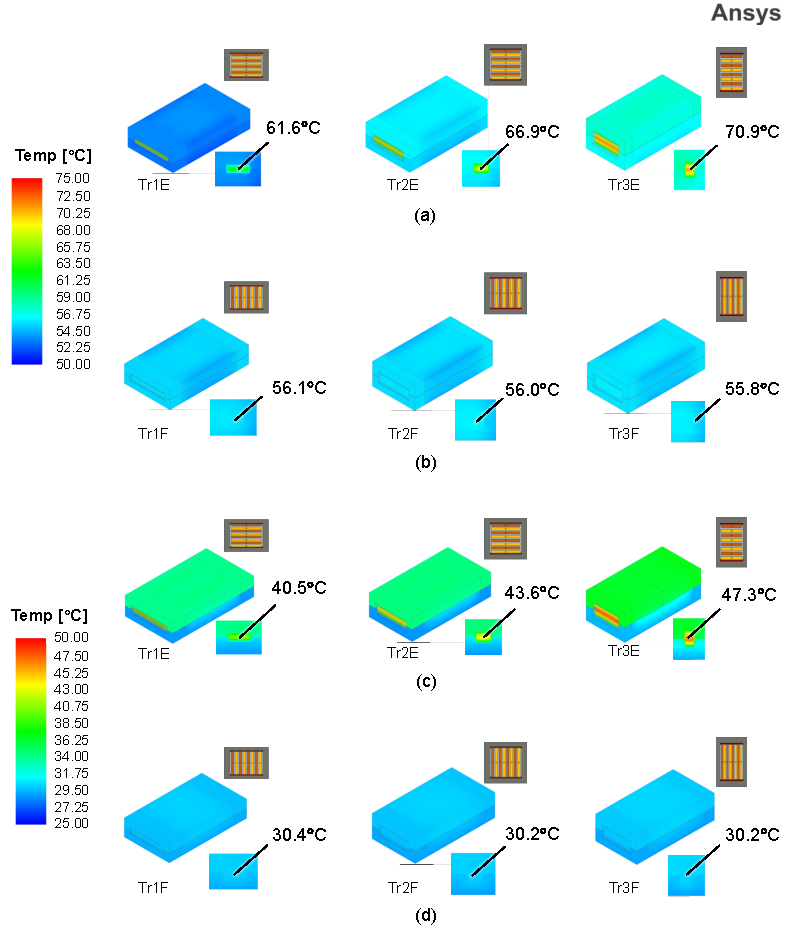
\includegraphics[width=\columnwidth]{figures_chapter4/compilation.pdf}%
    \caption{Simulated thermal distribution of the evaluated transformer models at 28.5 kHz and 25°C ambient temperature: (a) edgewise and (b) flatwise (proposed) configurations under natural cooling; (c) edgewise and (d) flatwise (proposed) configurations under forced-air cooling.}
    \label{fig:compilation}
\end{figure}

\begin{figure}[h!]
    \centering
    \subfloat[]{
        \centering
        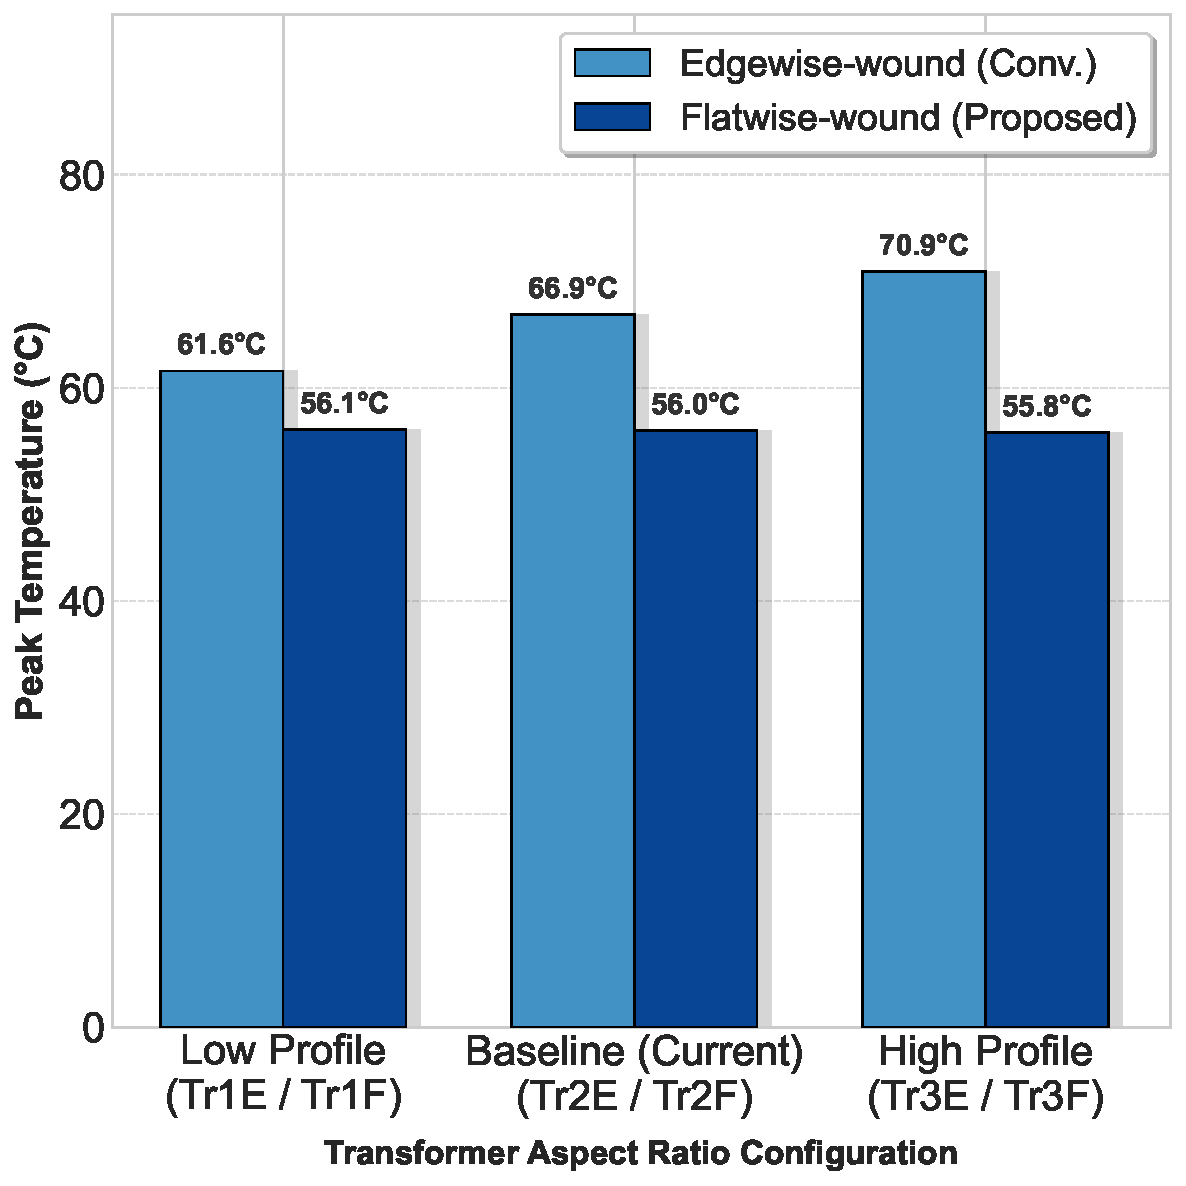
\includegraphics[width=0.45\columnwidth]{figures_chapter4/thermal_natural_grouped.pdf}
        \label{fig:compilation_natural}
    }
    \hfill
    \subfloat[]{
        \centering
        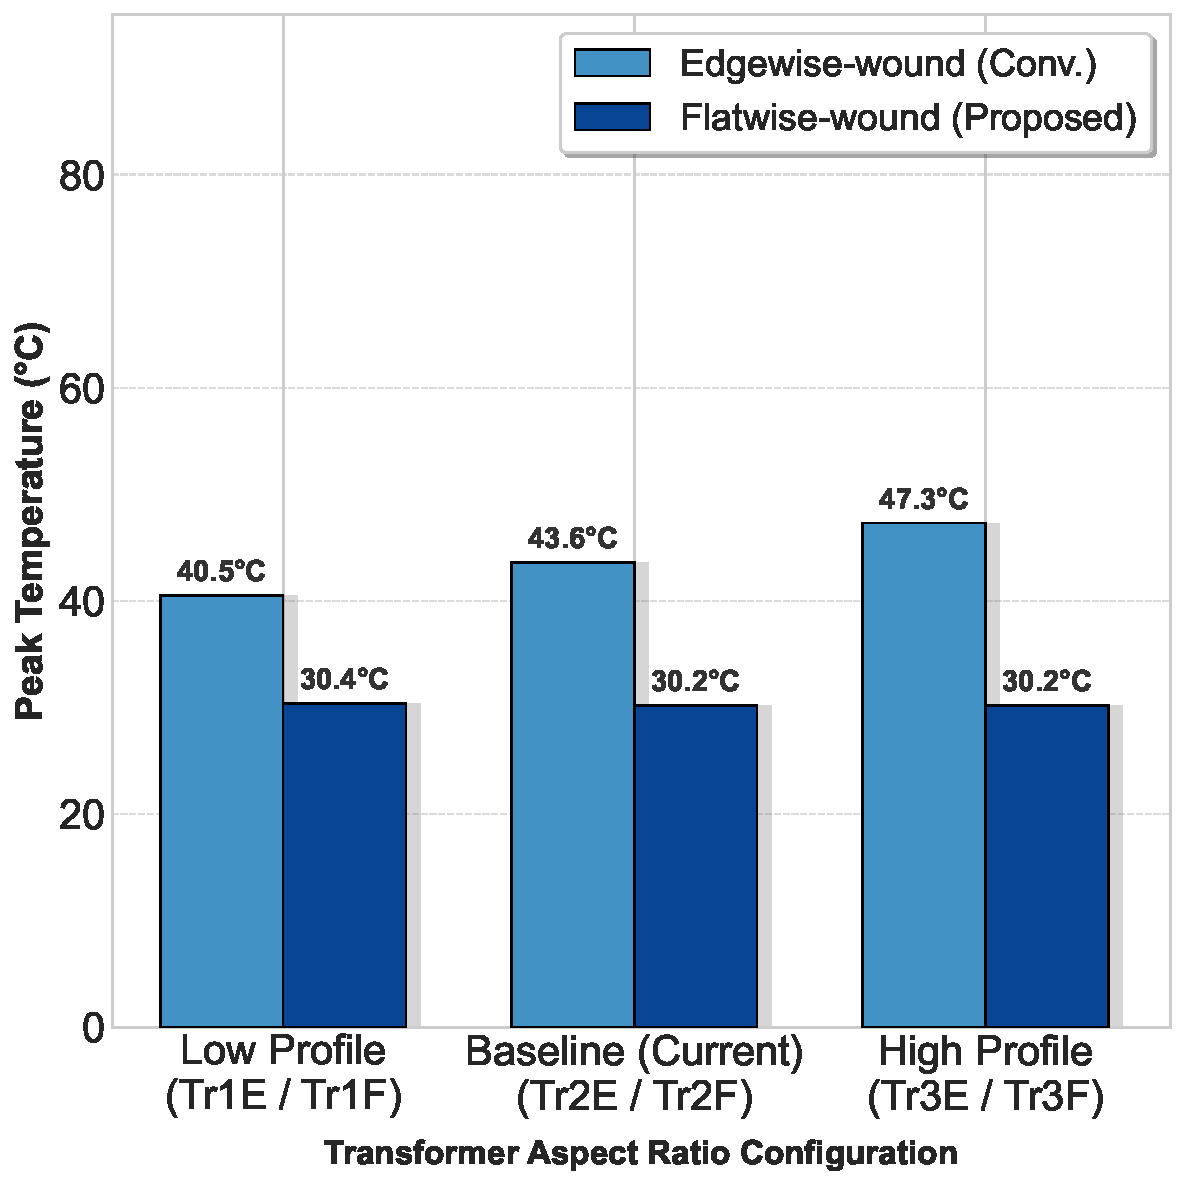
\includegraphics[width=0.45\columnwidth]{figures_chapter4/thermal_forced_grouped.pdf}
        \label{fig:compilation_forced}
    }
    \caption{Summary of peak temperatures of the evaluated transformer models at 28.5 kHz and 25°C ambient temperature: (a) edgewise and flatwise configurations under natural cooling; (b) edgewise and flatwise configurations under forced-air cooling.}
    \label{fig:summary}
\end{figure}

\begin{table}[h!]
\centering
\caption{Transformer Losses at Different Geometries}
\label{tab:transformer_losses}
% Reduces the horizontal white space between columns
% Standard IEEE table font size
\begin{tabular}{lcccccc}
\hline
\hline
\textbf{Loss} & \textbf{Tr1F} & \textbf{Tr2F} & \textbf{Tr3F} & \textbf{Tr1E} & \textbf{Tr2E} & \textbf{Tr3E} \\
\hline
Winding Losses (W)  & 2.5530 & 2.3270 & 2.2900 & 2.3990 & 2.2440 & 2.1620 \\
Core Losses (W)     & 0.8798 & 0.8715 & 0.8938 & 0.9316 & 0.8740 & 0.8900 \\
Aluminum Losses (W) & 0.1172 & 0.0902 & 0.0821 & 0.0916 & 0.0885 & 0.0874 \\
\hline
\textbf{Total Losses} (W)    & 3.5499 & 3.2891 & 3.2662 & 3.4219 & 3.2069 & 3.1395 \\
\hline
\hline
\end{tabular} 
\end{table}

The forced-air cooling scenario further confirmed this advantage. The edgewise models in Figure \ref{fig:compilation}c still exhibited heat being trapped in the windings, resulting in peaks of 40.5$^\circ$C to 47.3$^\circ$C. Moreover, as seen in Figure \ref{fig:compilation}d, the flatwise models again exhibited consistent performance, maintaining a low peak temperature of approximately 30.2$^\circ$C and a uniform temperature distribution. 

Ultimately, this comprehensive set of results highlights the profound thermal scalability of the flatwise geometry. In terms of electrical performance, the total power losses of both configurations remain practically equivalent. Noticeably, there is a spatial trade-off, as the radial stacking of the flatwise configuration inherently consumes more horizontal window space as the profile goes lower, which tends to increase the mean turn length (MTL). However, by fundamentally minimizing the internal series thermal resistance, the structure guarantees exceptional heat extraction even when integrated with practical, external cooling methods. This massive thermal headroom not only prevents localized hotspots but also unlocks the potential for further volumetric miniaturization of the transformer in high-power-density converter applications.

\section{Power Scalability}
While the 1~kW prototype and geometric sweep validate the fundamental heat extraction mechanism of the flatwise winding structure, High-Frequency Transformers (HFTs) deployed in modular SSTs and high-power DC--DC converters typically operate at tens to hundreds of kilowatts. Therefore, a power scalability analysis is conducted to evaluate the electromagnetic and thermal performance of the proposed transformer architecture as the rated power is scaled from 1~kW to 10~kW and 100~kW.

\subsection{Electrical Specifications and Scaling Assumptions}
To perform a rigorous and fair comparison across different power levels, the electrical parameters of the CLLC resonant converter are scaled such that the underlying circuit dynamics and resonant tank characteristics remain consistent. Specifically, as the output power $P_{\mathrm{o}}$ is increased by a factor of 10 (to 10~kW) and 100 (to 100~kW), both the input and output voltages $V_{\mathrm{in}}, V_{\mathrm{o}}$ and the input and output currents $I_{\mathrm{in}}, I_{\mathrm{o}}$ are scaled equally. 

By scaling voltage and current at the same rate as had been explained in Chapter \ref{sec:established}, the effective load resistance $R_{\mathrm{o}} = V_{\mathrm{o}}/I_{\mathrm{o}}$ and the equivalent AC resistance derived via First Harmonic Approximation (FHA) given by Eq. \ref{eq:Rac}
remain constant across all power levels. Consequently, the quality factor $Q$, inductance ratio $k = 10.0$, voltage gain curve $M$, and resonant tank components $C_{\mathrm{r1}} = C_{\mathrm{r2}} = 1.4~\mu\text{F}$, $L_{\mathrm{r1}} = L_{\mathrm{r2}} = 20.1~\mu\text{H}$, and $L_{\mathrm{m}} = 200~\mu\text{H}$ remain identical for the 1~kW, 10~kW, and 100~kW designs. The electrical specifications across the three power ratings are summarized in Table~\ref{tab:power_electrical_specs}. More insight behind this choice of parameters is explained in Chapter \ref{sec:established}. 

\begin{table}[h!]
\centering
\caption{Electrical Specifications for the Power Scalability Analysis}
\label{tab:power_electrical_specs}
\begin{tabular}{llccc}
\hline
\hline
\textbf{Parameter} & \textbf{Symbol} & \textbf{1 kW} & \textbf{10 kW} & \textbf{100 kW} \\
\hline
Input Voltage & $V_{\mathrm{in}}$ & 100 V & $316\text{ V } (\times\sqrt{10})$ & $1000\text{ V } (\times 10)$ \\
Output Voltage & $V_{\mathrm{o}}$ & 100 V & $316\text{ V } (\times\sqrt{10})$ & $1000\text{ V } (\times 10)$ \\
Output Current & $I_{\mathrm{o}}$ & 10 A & $31.6\text{ A } (\times\sqrt{10})$ & $100\text{ A } (\times 10)$ \\
Output Power & $P_{\mathrm{o}}$ & 1 kW & $10\text{ kW } (\times 10)$ & $100\text{ kW } (\times 100)$ \\
Switching Frequency & $f_{\mathrm{sw}}$ & 28.5 kHz & 28.5 kHz & 28.5 kHz \\
Resonant Frequency & $f_{\mathrm{r}}$ & 30.0 kHz & 30.0 kHz & 30.0 kHz \\
Dead Time & $t_{\mathrm{d}}$ & 360 ns & 360 ns & 360 ns \\
Resonant Capacitance & $C_{\mathrm{r1}}, C_{\mathrm{r2}}$ & $1.4~\mu\text{F}$ & $1.4~\mu\text{F}$ & $1.4~\mu\text{F}$ \\
Resonant Inductance & $L_{\mathrm{r1}}, L_{\mathrm{r2}}$ & $20.1~\mu\text{H}$ & $20.1~\mu\text{H}$ & $20.1~\mu\text{H}$ \\
Target Mag. Inductance & $L_{\mathrm{m}}$ & $200~\mu\text{H}$ & $200~\mu\text{H}$ & $200~\mu\text{H}$ \\
\hline
\hline
\end{tabular}
\end{table}

\subsection{Area-Product ($AP$) Sizing Guidelines}
To scale the physical geometry of the baseline square-window transformers (Tr2E and Tr2F, denoted here as Tr.~E-1 and Tr.~F-1) to 10~kW (Tr.~E-10 and Tr.~F-10) and 100~kW (Tr.~E-100 and Tr.~F-100), the Area-Product ($AP$) method is utilized[cite: 47, 53, 58]. The area product relates the physical window area $A_{\mathrm{w}}$ and magnetic core cross-sectional area $A_{\mathrm{c}}$ to the electrical and magnetic constraints of the converter[cite: 53, 54]:
\begin{equation}
    AP = A_{\mathrm{w}} \cdot A_{\mathrm{c}} = \frac{V_{\mathrm{in}}(I_{\mathrm{p,rms}} + I_{\mathrm{s,rms}})}{K_{\mathrm{f}} f_{\mathrm{sw}} B_{\mathrm{m}} J_{\mathrm{m}} K_{\mathrm{u}}} = \frac{2 P_{\mathrm{o}}}{4 f_{\mathrm{sw}} B_{\mathrm{m}} J_{\mathrm{m}} K_{\mathrm{u}}},
\end{equation}
where $K_{\mathrm{f}} = 4$ is the waveform coefficient for square-wave voltage excitation ($n = 1$, $D = 0.5$), $B_{\mathrm{m}}$ is the maximum core flux density, $J_{\mathrm{m}}$ is the current density, and $K_{\mathrm{u}}$ is the window utilization factor[cite: 53, 69, 70]. 

In this scaling procedure, $L_{\mathrm{m}}$, $B_{\mathrm{m}}$, $J_{\mathrm{m}}$, $K_{\mathrm{u}}$, and the number of turns $N_{\mathrm{p}}:N_{\mathrm{s}} = 8:8$ are held constant across all power levels[cite: 52, 55, 58]. Separating the area product into its constituent components yields[cite: 54]:
\begin{equation}
    A_{\mathrm{c}} \ge \frac{V_{\mathrm{in}}}{4 f_{\mathrm{sw}} N_{\mathrm{p}} B_{\mathrm{m}}}, \quad A_{\mathrm{w}} = \frac{N_{\mathrm{p}}(I_{\mathrm{p,rms}} + I_{\mathrm{s,rms}})}{J_{\mathrm{m}} K_{\mathrm{u}}}.
\end{equation}
Thus, the core cross-sectional area $A_{\mathrm{c}}$ is proportional to the operating voltage ($A_{\mathrm{c}} \propto V_{\mathrm{in}}$), whereas the window area $A_{\mathrm{w}}$ is proportional to the operating current ($A_{\mathrm{w}} \propto I$)[cite: 54]. Let $\lambda_V$ and $\lambda_I$ represent the one-dimensional (1D) linear scaling factors for the core and window dimensions, respectively[cite: 54]:
\begin{equation}
    A_{\mathrm{c,new}} = (\lambda_V w_{\mathrm{core,old}})(\lambda_V l_{\mathrm{core,old}}) = \lambda_V^2 A_{\mathrm{c,old}} \implies \lambda_V = \sqrt{\frac{V_{\mathrm{new}}}{V_{\mathrm{old}}}},
\end{equation}
\begin{equation}
    A_{\mathrm{w,new}} = (\lambda_I w_{\mathrm{win,old}})(\lambda_I l_{\mathrm{win,old}}) = \lambda_I^2 A_{\mathrm{w,old}} \implies \lambda_I = \sqrt{\frac{I_{\mathrm{new}}}{I_{\mathrm{old}}}}.
\end{equation}

Because voltage and current are scaled equally ($V_{\mathrm{new}}/V_{\mathrm{old}} = I_{\mathrm{new}}/I_{\mathrm{old}}$), the 1D scaling factors are identical ($\lambda_V = \lambda_I$), which preserves the square window aspect ratio ($l_{\mathrm{win}}/w_{\mathrm{win}} \approx 1.00$) and constant window utilization factor $K_{\mathrm{u}}$ across all power levels[cite: 51, 52, 55, 58]:
\begin{itemize}
    \item \textbf{Core Dimensions:} The center-leg ($l_{\mathrm{core}} \times w_{\mathrm{core}}$) and outer-leg ($l_{\mathrm{core}} \times 0.5w_{\mathrm{core}}$) dimensions are scaled linearly by $\lambda_V$[cite: 55, 56, 57].
    \item \textbf{Window and Conductor Dimensions:} The window width $w_{\mathrm{win}}$, window height $l_{\mathrm{win}}$, wire thickness $t$, clearances $d_{\mathrm{clear}}$, TIM thickness $d_{\mathrm{TIM}}$, and inter-turn insulation distance $d_{\mathrm{inter}}$ are scaled linearly by $\lambda_I$[cite: 52, 55, 56, 57].
    \item \textbf{Air Gap Length:} To maintain a constant magnetizing inductance $L_{\mathrm{m}} \approx \mu_0 N_{\mathrm{p}}^2 A_{\mathrm{c}} / l_{\mathrm{g}}$ as $A_{\mathrm{c}}$ increases by $\lambda_V^2$, the air gap length $l_{\mathrm{g}}$ is scaled proportionally to the voltage ratio ($\lambda_V^2$)[cite: 52, 55]:
    \begin{equation}
        l_{\mathrm{g,new}} = l_{\mathrm{g,old}} \frac{A_{\mathrm{c,new}}}{A_{\mathrm{c,old}}} = \lambda_V^2 l_{\mathrm{g,old}}.
    \end{equation}
\end{itemize}

The total area-product scaling factor is defined as $\lambda_{AP} = \lambda_V \cdot \lambda_I$[cite: 55]. Since transformer volume scales according to $Vol_{\mathrm{tr}} \propto P_{\mathrm{o}}^{3/4} \propto AP^{3/4}$, the overall three-dimensional volume of the scaled transformers increases by $\lambda_{AP}^{3/4}$[cite: 62, 69]. The resulting physical and electrical parameters for the 1~kW, 10~kW, and 100~kW transformer models are detailed in Table~\ref{tab:power_scaling_specs}[cite: 58, 62].

\begin{table}[h!]
\centering
\caption{Simulation Specifications and Dimensions for the Power Scalability Models[cite: 58, 62]}
\label{tab:power_scaling_specs}
\resizebox{\textwidth}{!}{%
\begin{tabular}{lcccccc}
\hline
\hline
\textbf{Parameter} & \textbf{Tr. F-1} & \textbf{Tr. F-10} & \textbf{Tr. F-100} & \textbf{Tr. E-1} & \textbf{Tr. E-10} & \textbf{Tr. E-100} \\
\hline
Rated Power $P_{\mathrm{o}}$ & 1 kW & 10 kW & 100 kW & 1 kW & 10 kW & 100 kW \\
Voltage Scaling Factor $\lambda_V$ & 1 & $\sqrt[4]{10}$ & $\sqrt{10}$ & 1 & $\sqrt[4]{10}$ & $\sqrt{10}$ \\
Current Scaling Factor $\lambda_I$ & 1 & $\sqrt[4]{10}$ & $\sqrt{10}$ & 1 & $\sqrt[4]{10}$ & $\sqrt{10}$ \\
$AP$ Scaling Factor $\lambda_{AP}$ & 1 & $\sqrt{10}$ & 10 & 1 & $\sqrt{10}$ & 10 \\
Wire Thickness $t$ (mm) & 0.30 & 0.53 & 0.95 & 0.30 & 0.53 & 0.95 \\
Aspect Ratio $l_{\mathrm{win}}/w_{\mathrm{win}}$ & $\sim$1.00 & $\sim$1.00 & $\sim$1.00 & $\sim$1.00 & $\sim$1.00 & $\sim$1.00 \\
Air Gap $l_{\mathrm{g}}$ (mm) & 0.10 & 0.32 & 1.00 & 0.10 & 0.32 & 1.00 \\
Mag. Inductance $L_{\mathrm{m}}$ ($\mu$H) & 200.00 & 208.11 & 216.49 & 200.00 & 207.36 & 215.24 \\
Dimensions $l_{\mathrm{tr}} \times w_{\mathrm{tr}} \times h_{\mathrm{tr}}$ (mm) & \makecell{67.46 $\times$ 36.60 \\ $\times$ 18.67} & \makecell{119.96 $\times$ 65.09 \\ $\times$ 33.20} & \makecell{213.33 $\times$ 115.74 \\ $\times$ 59.03} & \makecell{68.19 $\times$ 37.33 \\ $\times$ 18.30} & \makecell{121.27 $\times$ 66.39 \\ $\times$ 32.54} & \makecell{215.65 $\times$ 118.06 \\ $\times$ 57.87} \\
\hline
\hline
\end{tabular}%
}
\end{table}

\subsection{Electromagnetic-Thermal Simulation Results}
To provide a standardized, general representation of active cooling across all three power scales, each transformer is mounted via a bottom TIM layer onto a fixed $20^\circ\text{C}$ cold-plate boundary covering the bottom surface of the transformer, with the surrounding ambient air at $25^\circ\text{C}$[cite: 52, 59, 60, 61]. This boundary condition ensures that the cooling capability scales proportionally with the bottom footprint area of each transformer, guaranteeing a fair comparison between the edgewise and flatwise structures[cite: 52, 62].

The simulated temperature distributions for the 1~kW, 10~kW, and 100~kW models are illustrated in Figure~\ref{fig:power_thermal_dist}[cite: 59, 60, 61, 88, 89, 90], while the comparative summaries of peak winding temperatures and loss breakdowns are presented in Figure~\ref{fig:power_scalability_summary} and Table~\ref{tab:power_scaling_losses}[cite: 63, 88, 89, 90].


\begin{table}[h!]
\centering
\caption{Simulated Losses and Peak Winding Temperatures Across Scaled Power Ratings[cite: 59, 60, 61, 63, 88, 89, 90]}
\label{tab:power_scaling_losses}
\resizebox{\textwidth}{!}{%
\begin{tabular}{lcccccc}
\hline
\hline
\textbf{Metric} & \textbf{Tr. F-1} & \textbf{Tr. F-10} & \textbf{Tr. F-100} & \textbf{Tr. E-1} & \textbf{Tr. E-10} & \textbf{Tr. E-100} \\
\hline
Winding Losses $P_{\mathrm{wind}}$ (W) & 2.33 & 15.09 & 126.40 & 2.24 & 14.50 & 107.90 \\
Core Losses $P_{\mathrm{core}}$ (W) & 0.87 & 4.91 & 27.27 & 0.87 & 4.95 & 27.66 \\
Aluminum Losses $P_{\mathrm{Al}}$ (W) & 0.09 & 1.39 & 12.66 & 0.09 & 1.38 & 13.10 \\
\hline
\textbf{Total Losses (W)} & \textbf{3.29} & \textbf{21.39} & \textbf{166.33} & \textbf{3.21} & \textbf{20.83} & \textbf{148.66} \\
\hline
\textbf{Peak Winding Temp. ($^\circ$C)} & \textbf{21.2} & \textbf{24.2} & \textbf{37.0} & \textbf{36.8} & \textbf{78.2} & \textbf{210.6} \\
\hline
\hline
\end{tabular}%
}
\end{table}

As demonstrated in Table~\ref{tab:power_scaling_losses} and Figure~\ref{fig:power_scalability_summary}(a), the divergence in thermal performance between the two winding orientations becomes dramatically amplified as the power rating increases[cite: 63]:
\begin{itemize}
    \item \textbf{At 1~kW:} With the $20^\circ\text{C}$ bottom cold plate, the conventional edgewise transformer (Tr.~E-1) reaches a peak winding temperature of $36.8^\circ\text{C}$, whereas the proposed flatwise transformer (Tr.~F-1) remains at just $21.2^\circ\text{C}$ (only $1.2^\circ\text{C}$ above the cold-plate temperature)[cite: 52, 59, 88].
    \item \textbf{At 10~kW:} As total losses increase to approximately 21~W and the inter-turn insulation layers scale thicker by $\lambda_I = \sqrt[4]{10}$, the series thermal resistance of the edgewise winding traps heat in the upper turns, driving the peak temperature of Tr.~E-10 to $78.2^\circ\text{C}$[cite: 25, 56, 58, 60]. In stark contrast, the parallel heat conduction paths of the flatwise design (Tr.~F-10) restrict the peak winding temperature to $24.2^\circ\text{C}$[cite: 23, 60, 89].
    \item \textbf{At 100~kW:} At full SST module scale, the conventional edgewise design (Tr.~E-100) experiences severe thermal runaway, reaching an unsustainable peak winding temperature of $210.6^\circ\text{C}$ due to the cumulative thermal resistance of the stacked insulation layers and the increased vertical distance from the bottom cold plate[cite: 25, 52, 56, 61]. Conversely, the proposed flatwise-wound transformer (Tr.~F-100) maintains a remarkable peak winding temperature of only $37.0^\circ\text{C}$[cite: 61, 90].
\end{itemize}

Examining the loss breakdown in Figure~\ref{fig:power_scalability_summary}(b) and Table~\ref{tab:power_scaling_losses}, the flatwise configuration incurs a slightly higher AC winding loss at 100~kW ($126.40\text{ W}$ vs.\ $107.90\text{ W}$ for edgewise), resulting in a total loss of $166.33\text{ W}$ compared to $148.66\text{ W}$[cite: 63, 90]. This marginal increase (representing only a $0.018\%$ difference in overall efficiency at 100~kW) occurs because the conductor thickness scales to $t = 0.95\text{ mm}$ at 100~kW—approaching the skin depth limit at 28.5~kHz—and the vertical orientation of the flatwise turns experiences slightly higher fringing flux near the air gap[cite: 23, 27, 57, 58]. Nevertheless, delivering a $173.6^\circ\text{C}$ reduction in peak winding temperature at 100~kW in exchange for a negligible increase in conduction loss proves that the proposed flatwise-wound architecture is exceptionally well-suited for high-power, high-density SST applications[cite: 5, 61, 63].